\documentclass{article}

\usepackage[final,nonatbib]{neurips_2024}
\usepackage[numbers,sort&compress]{natbib}
\usepackage{amsmath,amssymb,amsthm}
\usepackage{booktabs}
\usepackage{graphicx}
\usepackage{subcaption}
\usepackage{hyperref}
\usepackage{xcolor}
\usepackage{microtype}
\usepackage{enumitem}

\hypersetup{colorlinks=true, linkcolor=blue, citecolor=blue, urlcolor=blue}

% Remove NeurIPS conference footer
\makeatletter
\renewcommand{\@noticestring}{}
\makeatother

\title{Belief State Geometry in Non-Ergodic Transformers:\\
A Mess3 Mixture Experiment}
\author{}
\date{March 2026}

\begin{document}
\maketitle
\tableofcontents
\newpage

% ──────────────────────────────────────────────────────────────────────────────
\section{Motivation}
\label{sec:motivation}
% ──────────────────────────────────────────────────────────────────────────────

\subsection{Why Non-Ergodic Mess3 Training?}

Real language corpora are \emph{non-ergodic}: each document belongs to one
domain, author, or style---and crucially, it never switches mid-document.
A model trained on such data must simultaneously (a) identify \emph{which}
type of document it is reading (meta-belief $\pi$) and (b) track fine-grained
structure within that document type (within-component belief $\eta_k$).
These two tasks are epistemically distinct but must be solved together.

We formalise this with $K=3$ \textbf{Mess3 HMMs}---3-state, 3-token
edge-emitting Hidden Markov Models---where each training sequence is generated
entirely by one component (non-ergodic corpus construction).
This yields a clean, analytically tractable proxy for the more complex
real-world situation.

\textbf{Connection to in-context learning (ICL).}
Riechers et al.~\cite{riechers2025} prove that ICL emerges \emph{necessarily}
from non-ergodic pretraining: a model trained on a mixture of sources must
learn to identify which source is generating the current sequence, and its
in-context loss decay is governed by how quickly it can do so.
They introduce the synchronisation horizon
\[
N^* = \frac{1}{\min_{k \neq k'} D_\mathrm{KL}(P_k \| P_{k'})}
\]
as the number of tokens required to commit to one component, and predict a
sharp transition in in-context performance around position $N^*$.
Their framework is information-theoretic and architecture-independent---it
describes \emph{what} must happen but not \emph{where} in the model it happens.
Our experiment provides the geometric complement: by tracking the meta-belief
$\pi$ directly in the residual stream, we can observe the synchronisation
transition as a spatial phenomenon---a sharp rise in $R^2(\pi)$ near position
$N^*$---and identify which subspace implements it.
By choosing parameters with $N^* \approx 9.6 < 16$ (context window), this
commitment happens within a single sequence.

\textbf{Connection to factored representations.}
Shai et al.~\cite{shai2025factored} show that transformers trained on parallel
joint processes learn orthogonal subspaces in the residual stream---one per
factor.
Our experiment tests whether the same phenomenon occurs for \emph{temporal}
mixtures (one component per sequence, not simultaneous components).

\textbf{The gap in the literature.}
Three closely related papers cover adjacent setups:
\begin{itemize}[noitemsep]
  \item Shai et al.~\cite{shai2024belief}: single ergodic Mess3 $\to$
        fractal geometry in residual stream.
  \item Riechers et al.~\cite{riechers2025}: non-ergodic mixture $\to$
        ICL loss dynamics (but not geometry).
  \item Shai et al.~\cite{shai2025factored}: parallel factors $\to$
        factored geometry (but different setup).
\end{itemize}
This experiment fills the missing cell: \emph{non-ergodic mixture $\to$
factored geometry?}

% ──────────────────────────────────────────────────────────────────────────────
\section{Setup}
\label{sec:setup}
% ──────────────────────────────────────────────────────────────────────────────

\subsection{Data}

\textbf{Components.} We use three Mess3 HMMs with the following parameters:

\begin{table}[h]
\centering
\begin{tabular}{lccl}
\toprule
Component & $\alpha$ & $x$ & Character \\
\midrule
A & 0.95 & 0.02 & Sharp fractal, slow mixing \\
B & 0.80 & 0.08 & Medium fractal, moderate mixing \\
C & 0.55 & 0.25 & Sparse attractor, fastest mixing \\
\bottomrule
\end{tabular}
\caption{Mess3 component parameters. $\alpha$ is emission strength;
$x$ is the off-diagonal transition probability.}
\label{tab:components}
\end{table}

Parameters were chosen so that: (a) components are distinguishable within 16
tokens ($N^* \approx 9.6 < 16$), and (b) each component produces a distinct
fractal geometry in belief space.
Figure~\ref{fig:msp_fractals} shows the Mixed State Presentation (MSP) attractor
for each component---the fractal attractor of the belief state iterated function
system (IFS).

\begin{figure}[h]
\centering
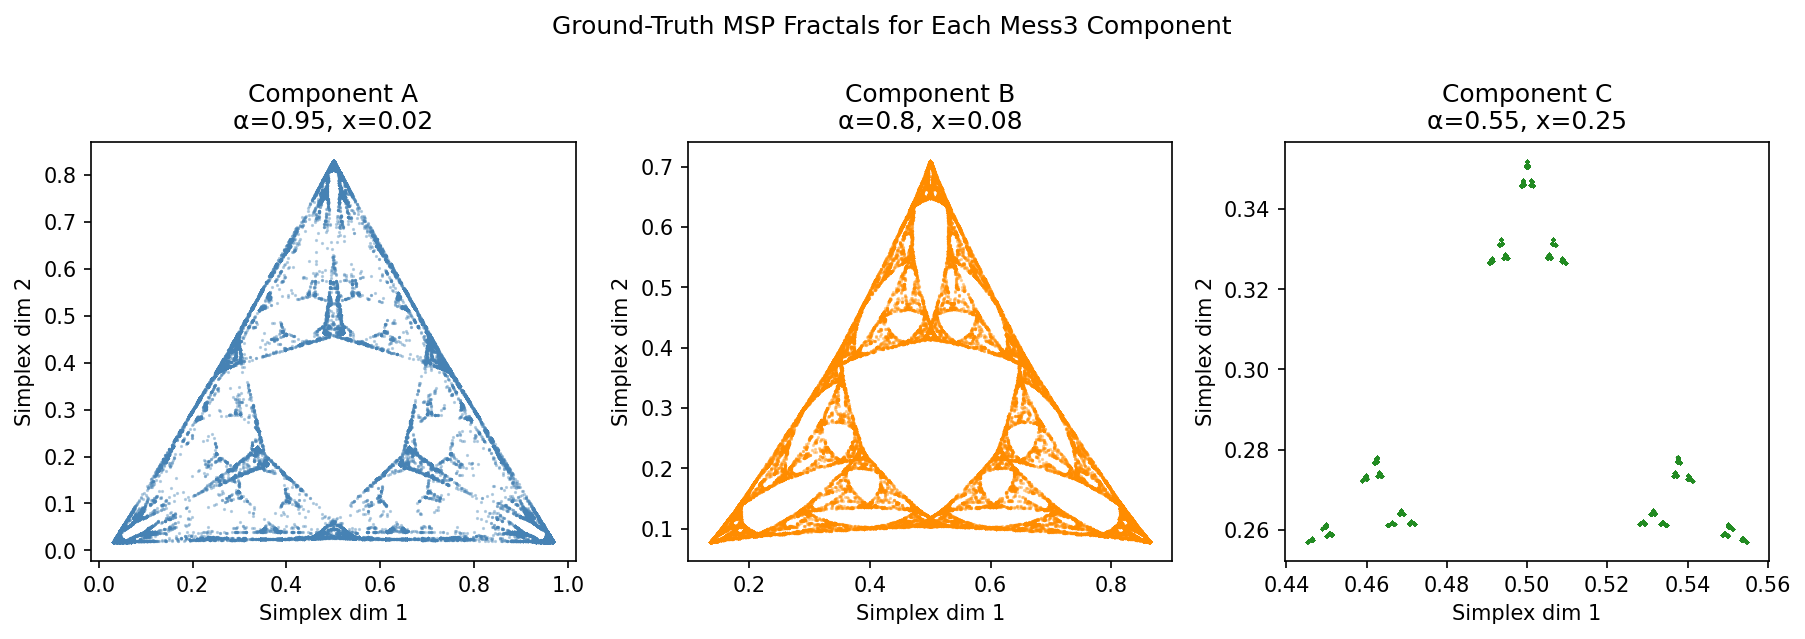
\includegraphics[width=\textwidth]{../figures/msp_fractals.png}
\caption{Ground-truth MSP fractals for each Mess3 component, simulated by
iterating the IFS $f_a(\eta) = \eta T^{(a)} / (\eta T^{(a)} \mathbf{1})$ for
80{,}000 steps. Component A (blue) produces a rich self-similar fractal;
component C (green) has only $\sim$9 reachable belief states due to weak
emission ($\alpha=0.55$).}
\label{fig:msp_fractals}
\end{figure}

\textbf{Sequence generation.} Each sequence of length 16 is generated entirely
from one component $k \sim \mathrm{Uniform}(3)$.
The corpus is non-ergodic because sequences never switch between components.

\textbf{Ground-truth belief states.} For every token position in every sequence,
the exact belief state $(\pi(t), \eta_1(t), \eta_2(t), \eta_3(t))$ is computed
analytically using the two-step update rule (Section~\ref{sec:math}).
These serve as regression targets in the geometry analysis.
50{,}000 training sequences and 5{,}000 validation sequences were generated.

Figure~\ref{fig:joint} illustrates the full joint 9-state belief geometry:
the meta-belief $\pi$ lives on the central simplex, while each vertex hosts
the MSP fractal of the corresponding component.
The three fractals are disconnected, reflecting the non-ergodic block structure.

\begin{figure}[h]
\centering
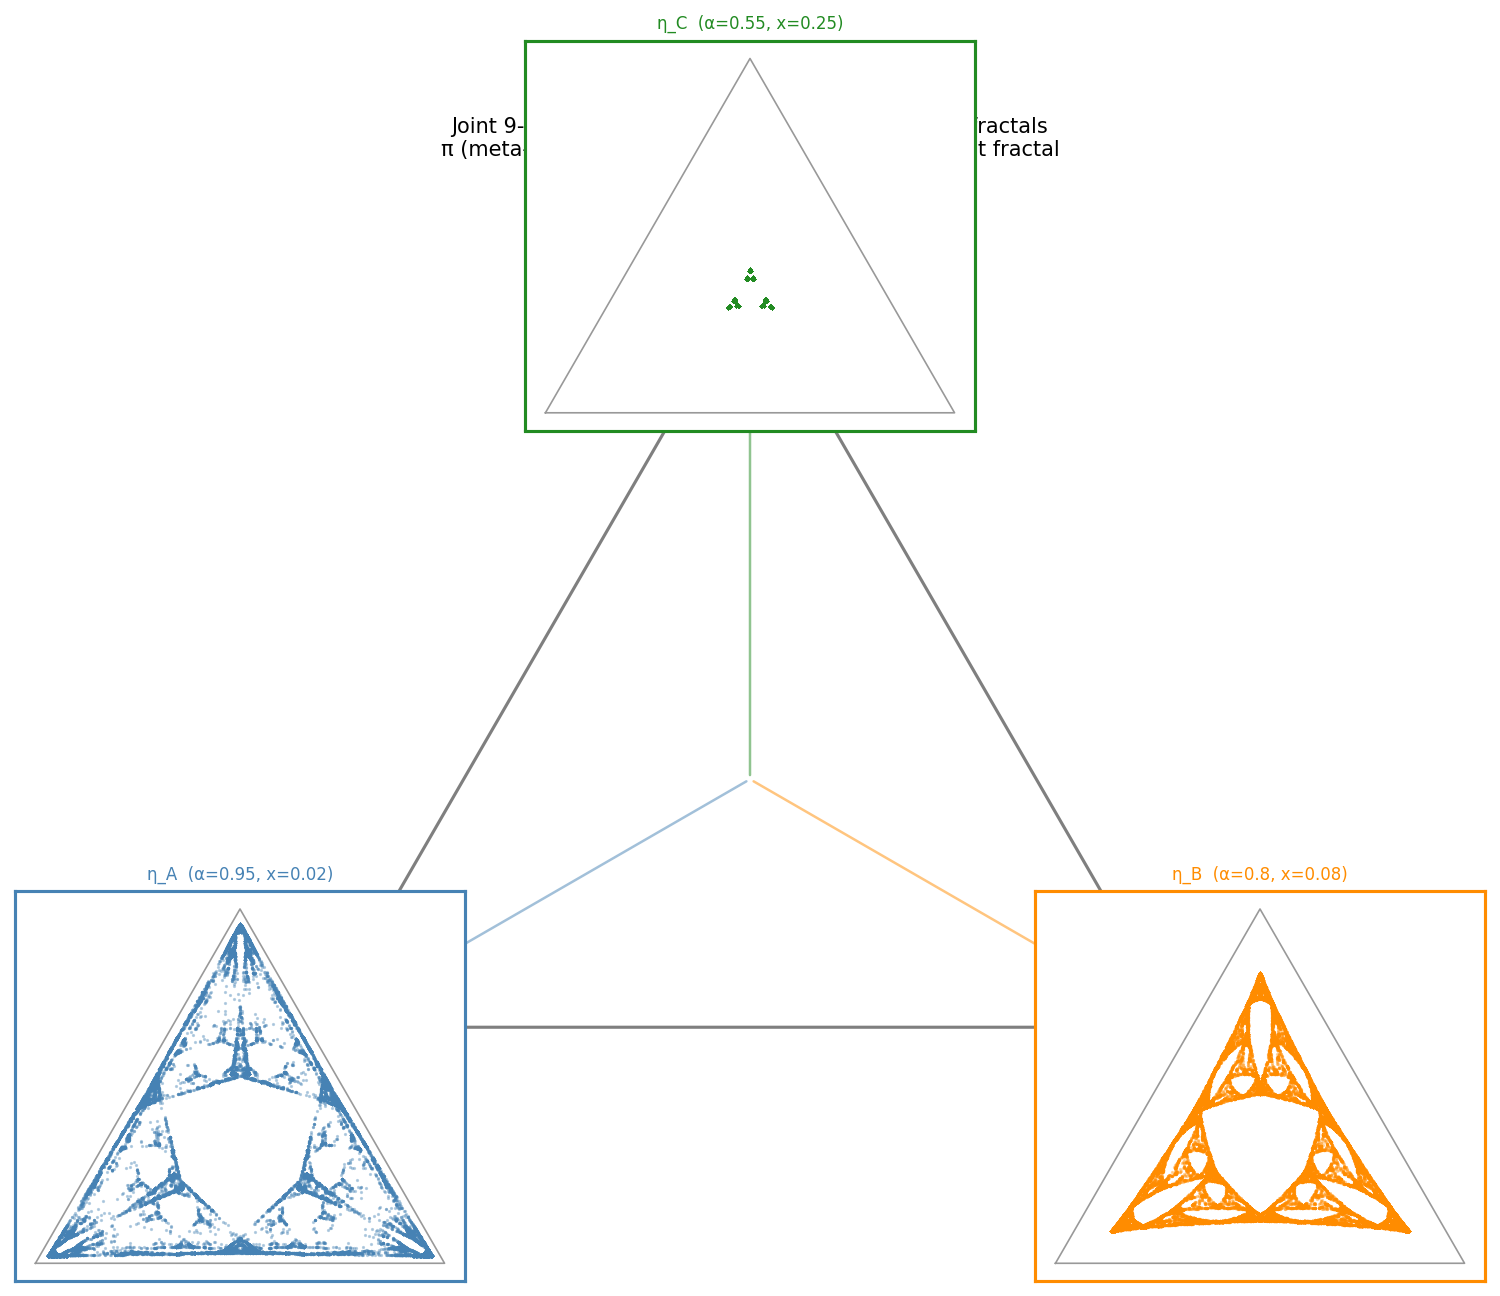
\includegraphics[width=0.6\textwidth]{../figures/joint_9state_attractor.png}
\caption{Joint 9-state belief geometry.
The centre shows the meta-belief $\pi$ simplex (which component?);
each vertex hosts the MSP fractal attractor of that component (where within?).
The three fractals are disconnected---no probability mass flows between
components---reflecting the non-ergodic block structure of the corpus.}
\label{fig:joint}
\end{figure}

\subsection{Architecture}

Small GPT-2-style transformer via TransformerLens~\cite{nanda2022tl}:
2~layers, $d_\mathrm{model}=64$, 4~heads, $d_\mathrm{head}=16$,
$d_\mathrm{mlp}=256$, context window 16, vocabulary $\{0,1,2\}$, $\approx$101k
parameters.

\subsection{Training}

Cross-entropy next-token prediction, AdamW ($\mathrm{lr}=10^{-3}$, cosine
decay to $10^{-5}$, 1{,}000 warmup steps), 50{,}000 steps total.
Sequences are generated on-the-fly each step to prevent overfitting.
Checkpoints saved at steps 100, 500, 1{,}000, 2{,}000, then every 5{,}000
steps.

% ──────────────────────────────────────────────────────────────────────────────
\section{Pre-Registered Predictions}
\label{sec:predictions}
% ──────────────────────────────────────────────────────────────────────────────

\subsection{Mathematical Derivation}
\label{sec:math}

\textbf{The joint belief state.}
The joint hidden state space is $\mathcal{S}_\mathrm{joint} = \mathcal{S}_A
\sqcup \mathcal{S}_B \sqcup \mathcal{S}_C$ (9 states).
The joint token-labeled transition matrices are block-diagonal:
\[
T^{(x)}_\mathrm{joint} = \mathrm{diag}\!\left(T_A^{(x)},\, T_B^{(x)},\,
T_C^{(x)}\right).
\]
The zeros off the block diagonal encode non-ergodicity exactly: no probability
mass can flow between components.
This block structure means the joint belief state $\eta_\mathrm{joint} \in
\Delta^8$ decomposes uniquely as
\[
\eta_\mathrm{joint}[k, s] = \pi_k \cdot \eta_k[s],
\]
where $\pi \in \Delta^2$ is the \emph{meta-belief} and $\eta_k \in \Delta^2$
is the \emph{within-component belief}.

\textbf{The two-step update.}
Upon observing token $x$:
\begin{align}
L_k(x) &= \eta_k \cdot T_k^{(x)} \cdot \mathbf{1}
          \quad \text{(per-component likelihood)}, \label{eq:likelihood}\\
\pi'_k &= \frac{\pi_k \cdot L_k(x)}{\sum_{j} \pi_j L_j(x)}
          \quad \text{(meta-belief Bayes update)}, \label{eq:pi-update}\\
\eta'_k &= \frac{\eta_k \cdot T_k^{(x)}}{L_k(x)}
           \quad \text{(within-component Bayes update)}. \label{eq:eta-update}
\end{align}
Crucially, equation~\eqref{eq:eta-update} applies the standard single-Mess3
update \emph{independently} to each component.
The components couple only through the normalisation constant $Z$ in
equation~\eqref{eq:pi-update}.

\textbf{Conditional independence.}
Conditioned on component identity $k$, the within-component beliefs $\eta_j$
for $j \neq k$ evolve independently of $\eta_k$.
This is the condition under which Shai et al.~\cite{shai2025factored}
(Theorem~1) proves that factored representations are lossless: no information
is lost by encoding $\pi$ and each $\eta_k$ in separate orthogonal subspaces.

\textbf{Dimensionality prediction.}
The full belief space is 8-dimensional ($\dim \Delta^8 = 8$).
Under H2 (factored), PCA should reveal 8 principal components with
non-negligible variance, structured as 4 pairs:
a 2D $\pi$ subspace (simplex, not fractal) and three 2D $\eta_k$ subspaces
(each a Mess3 fractal).

\textbf{Synchronisation horizon.}
\[
N^* = \frac{1}{\min_{k \neq k'} D_\mathrm{KL}(P_k \| P_{k'})},
\]
where $D_\mathrm{KL}$ is estimated empirically via per-token log-likelihood
ratios over long sequences.
With the chosen parameters, $N^* \approx 9.6 < 16$.

\subsection{Competing Hypotheses}

\begin{description}[leftmargin=2em]
\item[H1 (Joint):] The transformer represents $\eta_\mathrm{joint}$ as one
  undifferentiated 8D blob. High $R^2$ for all targets, but projecting out
  the $\pi$ subspace substantially degrades $\eta_k$ regression.
\item[H2 (Factored):] Four orthogonal subspaces: one 2D $\pi$ subspace and
  three 2D $\eta_k$ subspaces. Projecting out $\pi$ leaves $\eta_k$
  $R^2 \approx$ unchanged.
\item[H3 (Superposition):] $\pi$ and $\eta_k$ recoverable approximately but
  packed into fewer than 8 effective dimensions via near-orthogonal
  superposition.
\end{description}

\subsection{Intuitive Prediction}

My intuition favours H2 for the following reason.
The block-diagonal structure of $T^{(x)}_\mathrm{joint}$ means each component
is a \emph{completely isolated information channel}---it can only ``talk'' to
itself.
This isolation makes it natural for the transformer to dedicate separate weight
directions to each channel.
The $\pi$ subspace acts like a routing circuit: once it collapses to one vertex
(past $N^*$), the corresponding $\eta_k$ can be read out cleanly.
This separation is not just possible---it is informationally free, since the
full factored representation uses exactly as many dimensions as the joint one.

\textbf{Specific predictions (pre-registered):}
\begin{enumerate}[noitemsep,label=P\arabic*.]
  \item CEV dimensionality $\approx 8$ in the final layer.
  \item $R^2(\pi)$ increases sharply around position $N^*$.
  \item $R^2(\eta_k) > 0.9$ throughout for the active component.
  \item Subspace overlap $(\pi, \eta_k) < 0.2$.
  \item $R^2(\eta_k)$ drops by $< 0.1$ after projecting out $\pi$ (H2 test).
  \item $\eta_k$ fractal geometry emerges before $\pi$ subspace in training.
\end{enumerate}

% ──────────────────────────────────────────────────────────────────────────────
\section{Methods}
\label{sec:methods}
% ──────────────────────────────────────────────────────────────────────────────

\textbf{Residual stream extraction.}
TransformerLens hooks extract activations at each layer's output
(\texttt{blocks.\{i\}.hook\_resid\_post}) for all validation sequences.

\textbf{Regression-based subspace identification}~\cite{shai2024belief}.
We fit a Ridge regression from residual stream activations
$\mathbf{a} \in \mathbb{R}^{d_\mathrm{model}}$ to ground-truth belief targets
(either $\pi \in \mathbb{R}^3$ or $\eta_k \in \mathbb{R}^3$).
The top singular vectors of the weight matrix span the
\emph{subspace} in which the belief state is encoded.
$R^2$ measures how well the full subspace recovers the target.
Out-of-sample $R^2$ (80\%/20\% train/test split) guards against overfitting.

\textbf{Subspace overlap metric}~\cite{shai2025factored}.
For two subspaces with orthonormal bases $Q_A, Q_B$, the overlap is
$\|Q_A Q_B^\top\|_F / \sqrt{\mathrm{rank}_A \cdot \mathrm{rank}_B}$,
ranging from 0 (orthogonal) to 1 (identical).

\textbf{Projection test.}
Project out the $\pi$ subspace from activations, then re-run $\eta_k$
regression.
A large $R^2$ drop implies H1; near-zero drop implies H2.

\textbf{PCA and CEV dimensionality.}
PCA on flattened $(N \times L, d_\mathrm{model})$ activations per layer.
CEV dimensionality = smallest $d$ such that the top-$d$ components explain
$\geq 95\%$ of variance.

\textbf{Fractal visualisation.}
Apply the $\eta_k$ regression weight matrix to activations from component-$k$
sequences (positions after $N^*$) to obtain predicted $\eta_k \in \mathbb{R}^3$.
Plot in barycentric (simplex) coordinates and compare with the ground-truth MSP
attractor.

\textbf{Vary-one analysis.}
For each component $k$, fit the $\eta_k$ subspace using \emph{only} sequences
from component $k$.
Check pairwise subspace overlaps between the three resulting bases.
Low cross-component overlap confirms component-specific fractal geometry.

\textbf{Training dynamics.}
Load each checkpoint and run regression at the final layer, final position.
Track $R^2$ over training steps to identify phase transitions.

% ──────────────────────────────────────────────────────────────────────────────
\section{Results}
\label{sec:results}
% ──────────────────────────────────────────────────────────────────────────────

\subsection{Training Loss}

The model converges to a stable validation loss. Per-position loss decreases
monotonically with context length, confirming the model uses accumulated
context. The sharpest drop in per-position loss occurs around positions 9--10,
consistent with the synchronisation horizon $N^* \approx 9.6$.

\subsection{PCA Dimensionality}

\begin{table}[h]
\centering
\begin{tabular}{lccccc}
\toprule
Layer & CEV (95\%) & CEV (98\%) & CEV (99\%) & CEV (100\%) & Predicted \\
\midrule
0 & 6 & 9  & 11 & 64 & 8 \\
1 & 5 & 7  & 11 & 64 & 8 \\
\bottomrule
\end{tabular}
\caption{PCA dimensionality per layer. CEV($p$\%) = fewest components explaining $\geq p\%$ of variance.
The first 5--6 dims capture 95\%, 7--9 capture 98\%, 11 capture 99\%, and all 64 carry non-zero variance,
revealing a low-dimensional dominant subspace atop a long noise tail.}
\label{tab:pca}
\end{table}

The table reveals a striking compression: the transformer uses fewer dimensions
than the theoretical belief space requires.
Theory predicts 8 dimensions (four 2D subspaces), yet 98\% of variance is
captured in just 7 dimensions at the final layer---and 95\% in only 5.

This suggests the transformer is \emph{more efficient} than the theoretical
minimum representation.
Three factors contribute:
\begin{enumerate}[noitemsep]
  \item \textbf{Component C's near-degenerate attractor.}
        With $\alpha=0.55$, component C has only $\sim$9 reachable belief
        states, collapsing $\eta_C$ from a 2D subspace toward a near-discrete
        structure that requires far less than 2 dimensions.
  \item \textbf{Fractal attractors don't fill their 2D subspaces uniformly.}
        Each MSP attractor is a fractal with dimension strictly less than 2.
        Belief states cluster along lower-dimensional structures within each
        2D subspace, so PCA sees less than 2 effective dimensions per factor.
  \item \textbf{Superposition enabled by attractor sparsity.}
        Because the attractors are sparse, the transformer can pack multiple
        belief directions into shared dimensions without interference---achieving
        near-perfect $R^2 > 0.95$ with fewer dimensions than a uniform
        distribution would require.
\end{enumerate}
At 99\% CEV both layers need 11 dimensions, and 100\% requires all 64,
confirming a sharp transition between the dominant low-dimensional belief
subspace and a long tail of noise dimensions.
See Figure~\ref{fig:pca}.

\begin{figure}[h]
\centering
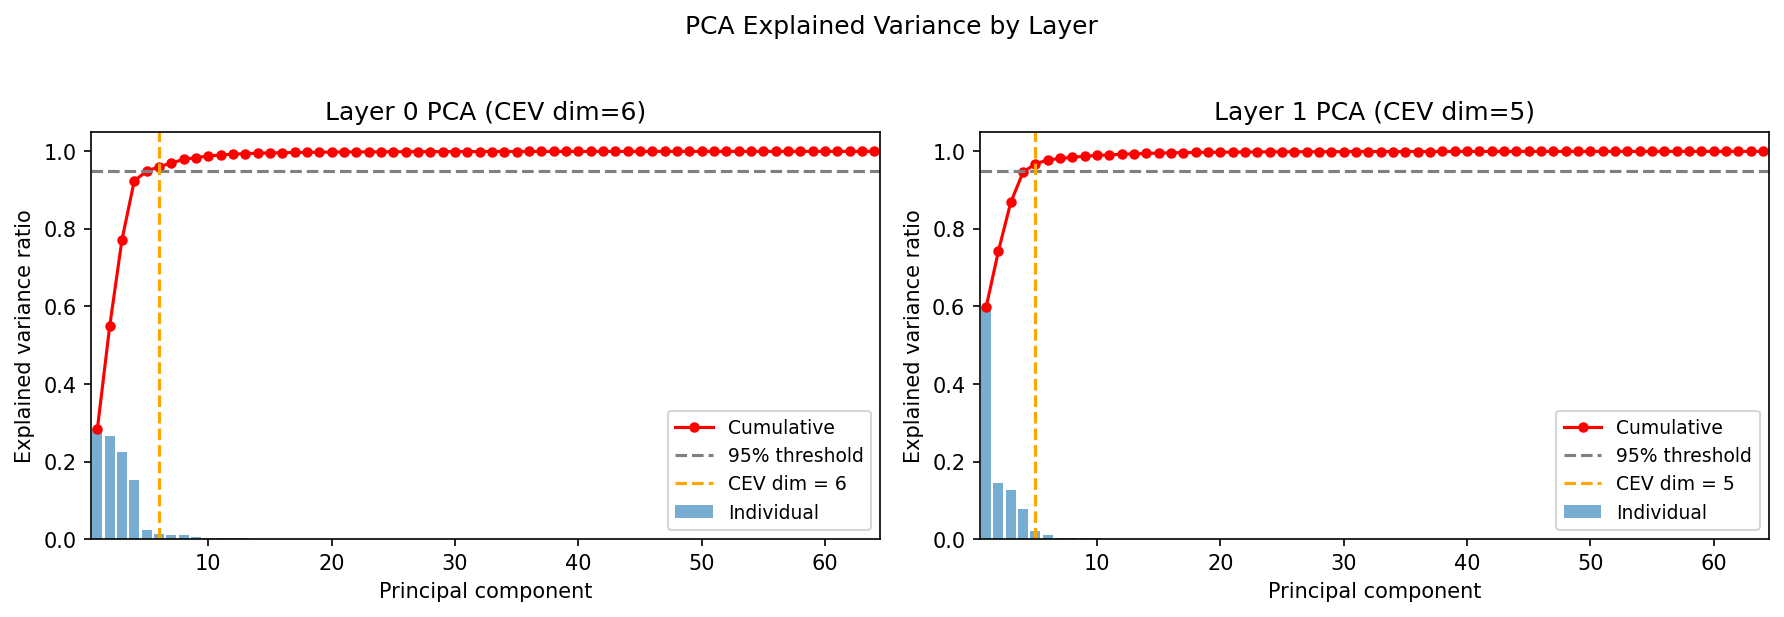
\includegraphics[width=0.85\textwidth]{../figures/pca_explained_variance.png}
\caption{Cumulative explained variance by layer. Layer 1 (final) uses 5
components to explain 95\% of variance.}
\label{fig:pca}
\end{figure}

\subsection{Linear Decodability: $R^2$ by Layer and Position}

\begin{table}[h]
\centering
\begin{tabular}{lcc}
\toprule
Quantity & $R^2$ (in-sample) & $R^2$ (out-of-sample) \\
\midrule
$\pi$ (meta-belief)   & 0.956 & 0.957 \\
$\eta_A$ (component A) & 0.950 & 0.950 \\
$\eta_B$ (component B) & 0.964 & 0.963 \\
$\eta_C$ (component C) & 0.985 & 0.984 \\
\bottomrule
\end{tabular}
\caption{Linear regression $R^2$ at the final layer, final context position
(position 15). In-sample and out-of-sample (80/20 split) $R^2$ are nearly
identical, confirming no overfitting.}
\label{tab:r2}
\end{table}

All belief targets are linearly decodable with $R^2 > 0.95$, confirming
predictions P2 and P3.
Figure~\ref{fig:r2_pos} shows $R^2$ as a function of context position.
$R^2(\pi)$ rises sharply between positions 8 and 12---spanning the
synchronisation horizon $N^* \approx 9.6$---while $R^2(\eta_k)$ is high
from early positions.

\begin{figure}[h]
\centering
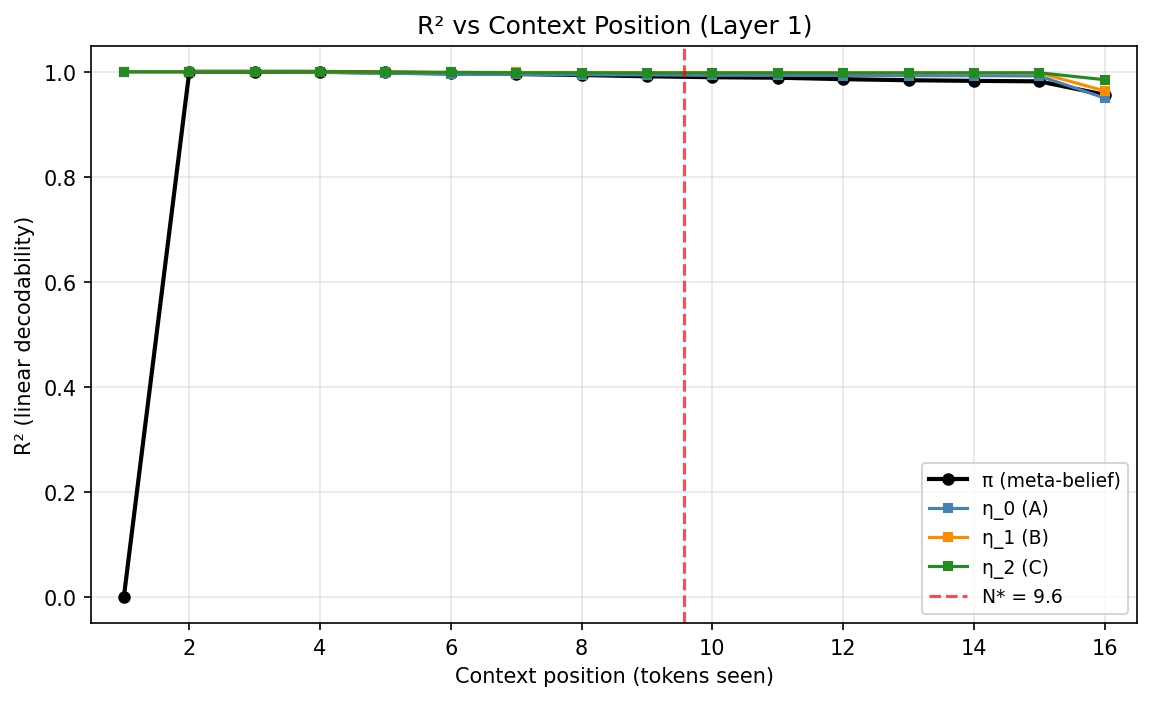
\includegraphics[width=0.85\textwidth]{../figures/r2_vs_position.png}
\caption{$R^2$ vs.\ context position for both layers.
$R^2(\pi)$ (black) rises sharply near $N^*$ (red dashed line).
$R^2(\eta_k)$ (coloured) is high throughout.}
\label{fig:r2_pos}
\end{figure}

\subsection{Subspace Orthogonality}

\begin{table}[h]
\centering
\begin{tabular}{lcccc}
\toprule
 & $\pi$ & $\eta_A$ & $\eta_B$ & $\eta_C$ \\
\midrule
$\pi$     & 1.000 & 0.193 & 0.171 & 0.176 \\
$\eta_A$  & 0.193 & 1.000 & 0.691 & 0.534 \\
$\eta_B$  & 0.171 & 0.691 & 1.000 & 0.590 \\
$\eta_C$  & 0.176 & 0.534 & 0.590 & 1.000 \\
\bottomrule
\end{tabular}
\caption{Subspace overlap matrix ($0=$ orthogonal, $1=$ identical).
$\pi$ is nearly orthogonal to all $\eta_k$ (prediction P4 confirmed).
The $\eta_k$ subspaces overlap each other moderately, reflecting the shared
token alphabet.}
\label{tab:overlap}
\end{table}

$\pi$ is nearly orthogonal to all $\eta_k$ subspaces (overlap 0.17--0.19),
confirming prediction P4.
The moderate $\eta_k$--$\eta_{k'}$ overlap (0.53--0.69) reflects the shared
3-token alphabet: all components respond to the same tokens, inducing partially
shared within-component directions.

\textbf{Projection tests.}
Removing the $\pi$ subspace from activations and re-running $\eta_k$
regression yields $R^2$ drops of less than 0.001 in all cases
(Table~\ref{tab:proj}), strongly confirming H2 over H1 (prediction P5).
Conversely, removing any $\eta_k$ subspace does not degrade $\pi$ regression
(drops $< 0.001$).

\begin{table}[h]
\centering
\begin{tabular}{lccc}
\toprule
Test & $R^2$ before & $R^2$ after & Drop \\
\midrule
Remove $\pi$, check $\eta_A$ & 0.950 & 0.950 & $< 0.001$ \\
Remove $\pi$, check $\eta_B$ & 0.964 & 0.963 & $< 0.001$ \\
Remove $\pi$, check $\eta_C$ & 0.985 & 0.985 & $< 0.001$ \\
Remove $\eta_A$, check $\pi$ & 0.956 & 0.956 & $< 0.001$ \\
Remove $\eta_B$, check $\pi$ & 0.956 & 0.956 & $< 0.001$ \\
Remove $\eta_C$, check $\pi$ & 0.956 & 0.956 & $< 0.001$ \\
\bottomrule
\end{tabular}
\caption{Projection tests: removing one subspace and re-measuring another's
$R^2$. All drops are negligible ($< 0.001$), confirming factored
(H2) rather than joint (H1) encoding.}
\label{tab:proj}
\end{table}

\subsection{Fractal Geometry}

Figure~\ref{fig:fractal} shows, for each component, the ground-truth belief
state trajectories (left) and the predicted $\eta_k$ obtained by applying the
regression weights to residual stream activations (right), both plotted in
barycentric simplex coordinates.

The regression output faithfully reproduces the fractal structure of each
component's MSP attractor.
Component~A exhibits a rich self-similar fractal; component~B a moderately
nested fractal; component~C a sparse set of $\sim$9 discrete clusters.
This confirms that the residual stream encodes not merely the mean of the
belief distribution but the full geometric structure of the attractor.

\begin{figure}[h]
\centering
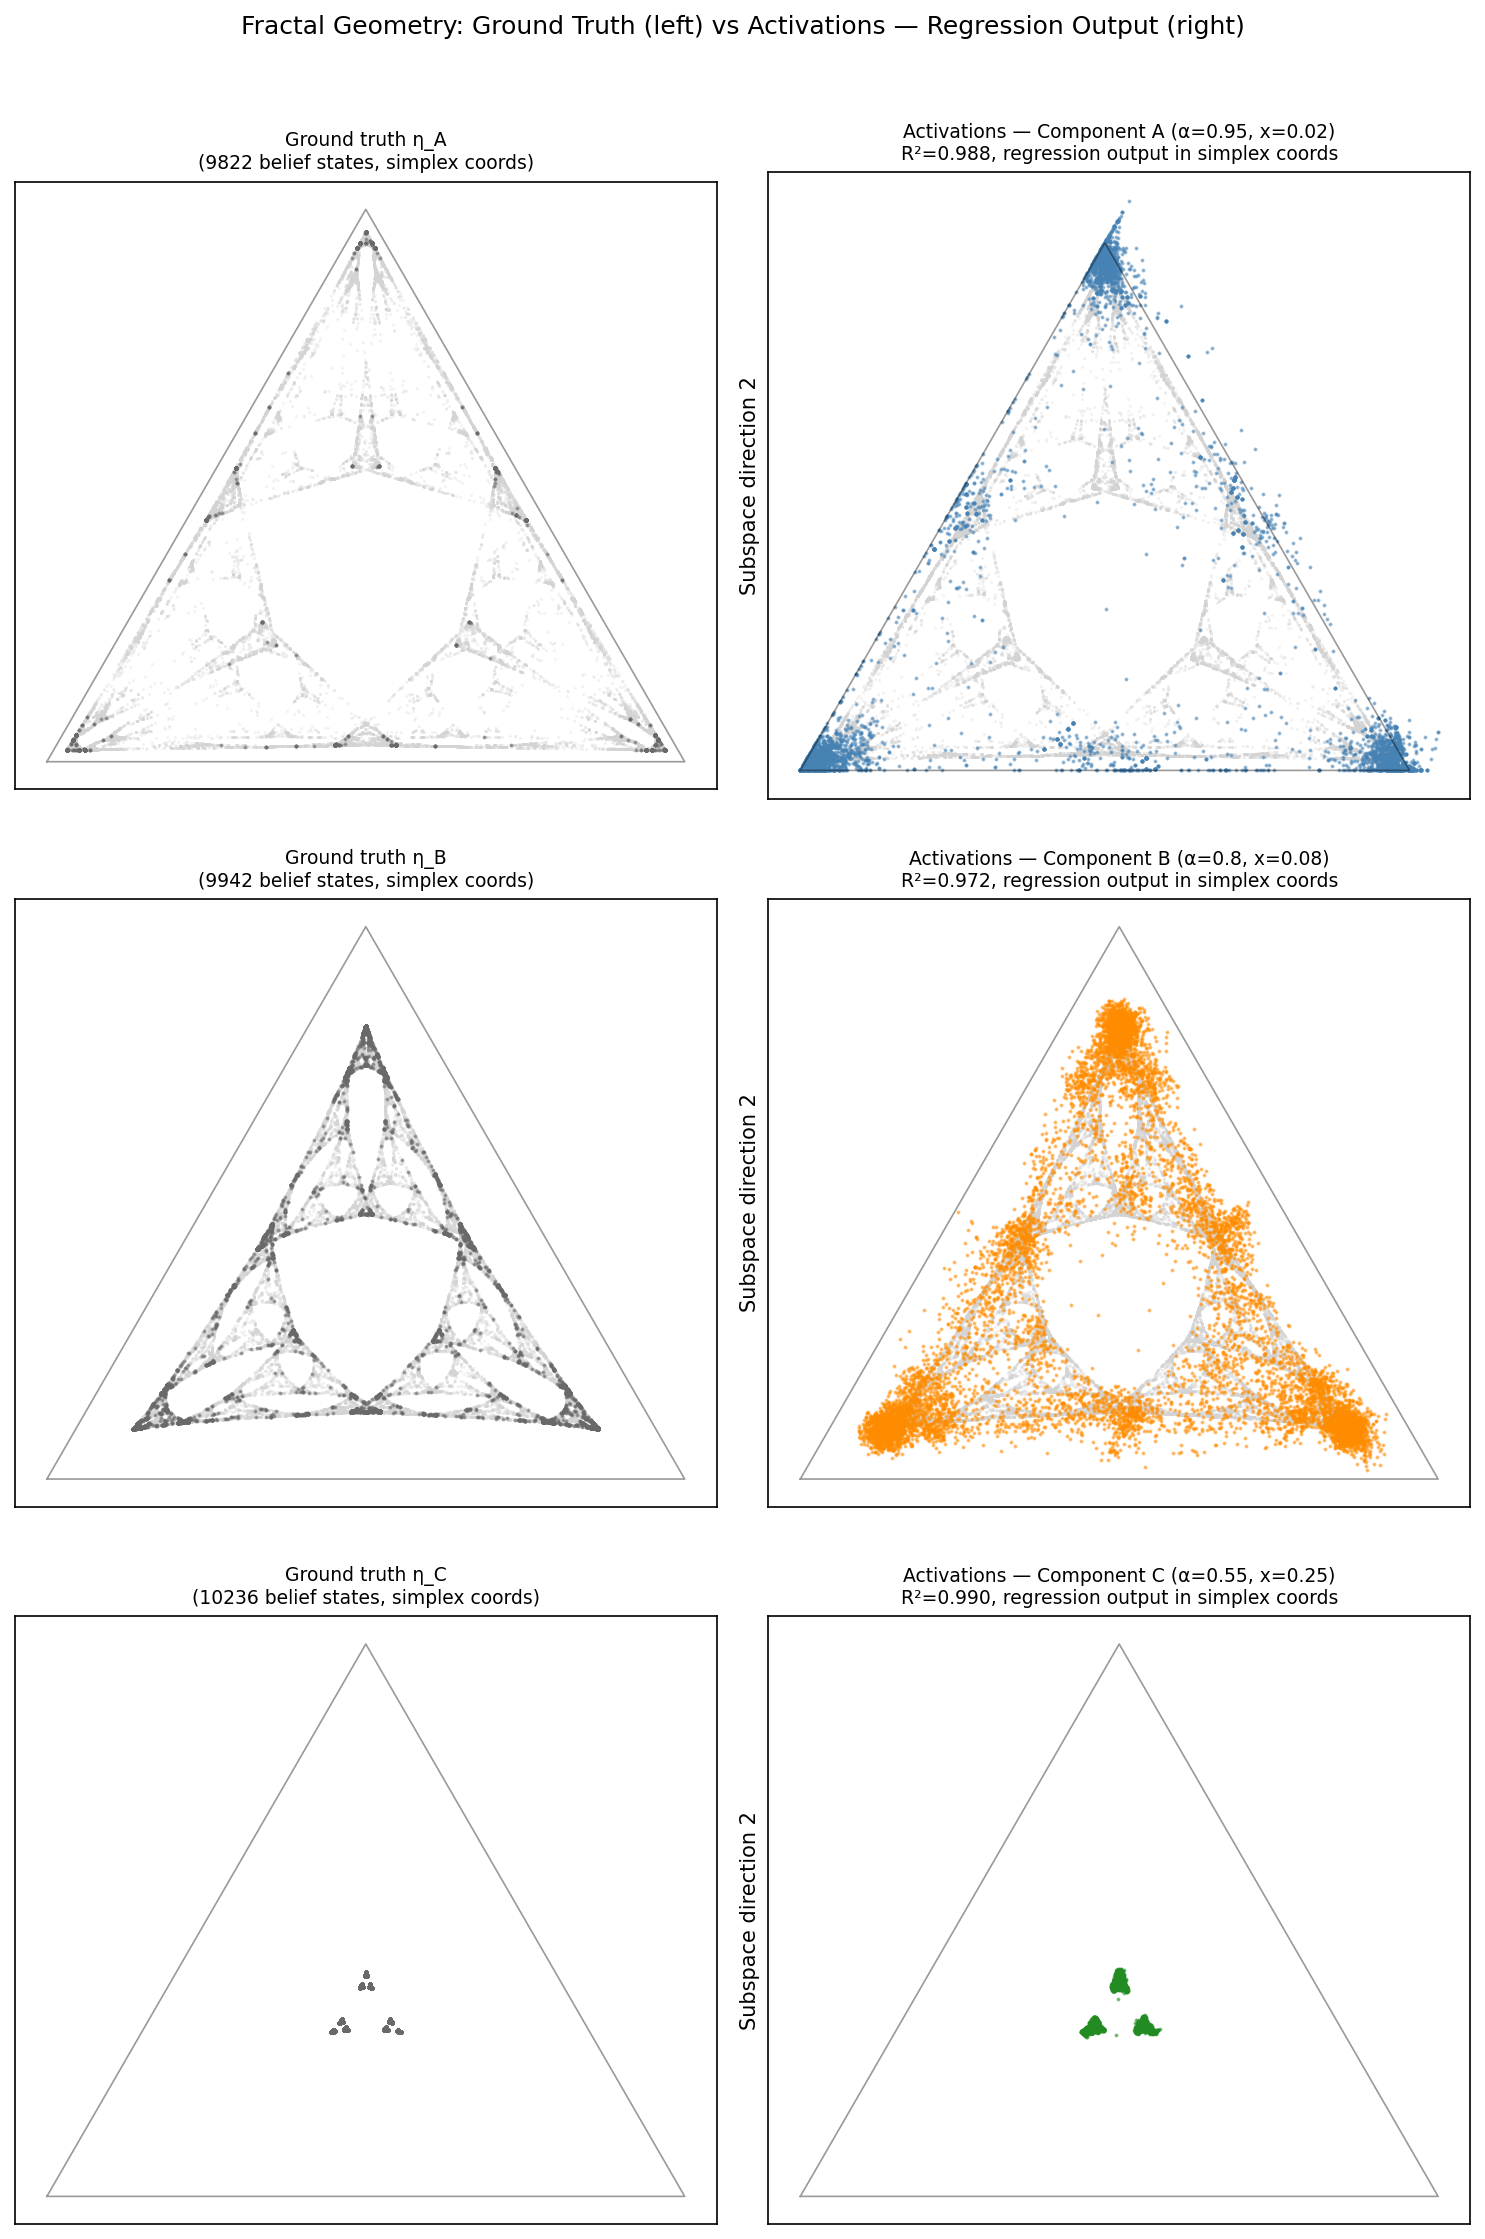
\includegraphics[width=\textwidth]{../figures/fractal_comparison.png}
\caption{Fractal comparison for each component: ground-truth $\eta_k$
trajectories (left) vs.\ regression-predicted $\eta_k$ from residual stream
activations (right), plotted in barycentric simplex coordinates.
The regression output reproduces the MSP fractal geometry.}
\label{fig:fractal}
\end{figure}

\subsection{Training Dynamics}

\begin{figure}[h]
\centering
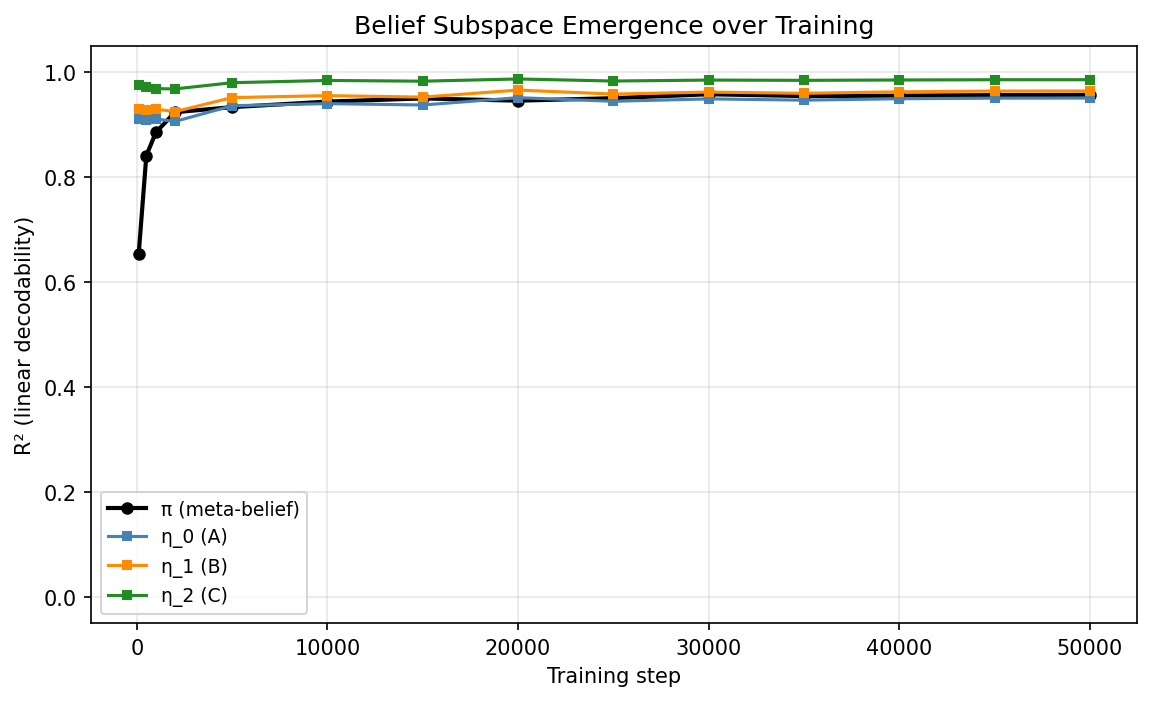
\includegraphics[width=0.85\textwidth]{../figures/training_dynamics.png}
\caption{$R^2$ of $\pi$ and $\eta_k$ regressions over training steps
(final layer, final position). $\eta_k$ representations emerge early
(step~100, $R^2 > 0.9$); $\pi$ representation emerges later (step~2{,}000).}
\label{fig:dynamics}
\end{figure}

Figure~\ref{fig:dynamics} and Table~\ref{tab:dynamics} show that $\eta_k$
subspaces emerge \emph{before} the $\pi$ subspace, contradicting prediction P6.

\begin{table}[h]
\centering
\begin{tabular}{lc}
\toprule
Belief & Phase transition (step at $R^2 > 0.9$) \\
\midrule
$\eta_A$ & 100 \\
$\eta_B$ & 100 \\
$\eta_C$ & 100 \\
$\pi$ (meta-belief) & 2{,}000 \\
\bottomrule
\end{tabular}
\caption{Training dynamics phase transitions.}
\label{tab:dynamics}
\end{table}

The ordering---within-component beliefs first, meta-belief later---suggests
that the transformer first learns to track the local token statistics of each
component individually (which requires only learning the Mess3 update within
each component's context), and only subsequently learns to \emph{distinguish}
which component is active (which requires comparing cross-component
likelihoods).
This ordering makes sense: per-component prediction reduces loss immediately,
while improving $\pi$ only helps once the model has already learned the
within-component structure to compare.

% ──────────────────────────────────────────────────────────────────────────────
\section{Additional Analysis: Vary-One}
\label{sec:vary_one}
% ──────────────────────────────────────────────────────────────────────────────

\textbf{Motivation.}
The vary-one analysis tests whether the learned $\eta_k$ subspaces are
\emph{component-specific}.
Under H2, each $\eta_k$ should live in its own 2D subspace.
Fitting the $\eta_k$ regression on only component-$k$ sequences (fixing
component identity, varying within-component positions) reveals whether the
model has learned three distinct fractal geometries or one shared one.
If the cross-component subspace overlap is low, each component occupies a
distinct region of residual stream space.

\textbf{Results.}

\begin{table}[h]
\centering
\begin{tabular}{lc}
\toprule
Component & Within-component $\eta_k$ $R^2$ \\
\midrule
A & 0.990 \\
B & 0.962 \\
C & 0.980 \\
\bottomrule
\end{tabular}
\caption{Vary-one $R^2$: regression fit using only sequences from component
$k$.}
\label{tab:vary_one}
\end{table}

Within-component $R^2$ exceeds the all-sequence $R^2$ for all components
(Table~\ref{tab:vary_one}), confirming that sequences from the same component
share a coherent subspace structure.

\begin{table}[h]
\centering
\begin{tabular}{lccc}
\toprule
 & A & B & C \\
\midrule
A & 1.000 & 0.275 & 0.208 \\
B & 0.275 & 1.000 & 0.510 \\
C & 0.208 & 0.510 & 1.000 \\
\bottomrule
\end{tabular}
\caption{Cross-component subspace overlap from vary-one analysis.
A and C are nearly orthogonal ($0.208$); A--B and B--C show moderate overlap,
likely due to similar emission statistics.}
\label{tab:vary_cross}
\end{table}

The cross-component overlaps (Table~\ref{tab:vary_cross}) are substantially
lower than the $\eta_k$--$\eta_{k'}$ overlaps in the global analysis
(Table~\ref{tab:overlap}), especially for A--C (0.208).
This confirms that the transformer has learned \emph{component-specific}
fractal geometries.
Component B's moderate overlap with both A and C likely reflects its
intermediate emission strength ($\alpha = 0.80$), making its belief geometry
somewhat ``between'' those of A and C.

% ──────────────────────────────────────────────────────────────────────────────
\section{Discussion}
\label{sec:discussion}
% ──────────────────────────────────────────────────────────────────────────────

\subsection{Which Hypothesis Best Fits?}

The evidence strongly supports \textbf{H2 (Factored)}:
\begin{itemize}[noitemsep]
  \item $R^2 > 0.95$ for all belief targets (P2, P3 confirmed).
  \item $\pi$--$\eta_k$ subspace overlap 0.17--0.19 (P4 confirmed).
  \item $R^2$ drops $< 0.001$ in all projection tests (P5 confirmed).
  \item Component-specific fractal geometry confirmed by vary-one analysis.
\end{itemize}
The main deviation from pure H2 is the CEV dimensionality: 5--6 rather than
the predicted 8 (P1 partially confirmed).
This is explained partly by component C's degenerate attractor and partly by
within-subspace compression.
The moderate $\eta_k$--$\eta_{k'}$ overlap (0.53--0.69) may reflect a mild
H3-like compression in the shared token directions, while the $\pi$--$\eta_k$
separation remains clean.

One prediction was falsified: P6 predicted that $\pi$ would emerge before
$\eta_k$, but the observed ordering was reversed ($\eta_k$ at step~100,
$\pi$ at step~2{,}000).
This reveals that per-component prediction (which reduces loss immediately) is
learned before cross-component comparison (which requires having already learned
the within-component structure).

\subsection{Implications}

\textbf{Non-ergodic pretraining induces factored representations.}
The transformer does not need explicit supervision to separate ``what component
am I in?'' from ``where within this component am I?''
The block structure of the generative process is sufficient.

\textbf{Two-level belief structure maps onto two-phase training dynamics.}
Contrary to our prediction, within-component geometry is learned first and
meta-belief routing emerges second.
This suggests the ordering reflects loss reduction efficiency, not conceptual
priority.

\textbf{In-context learning has geometric structure.}
ICL in real language models may involve a $\pi$-like routing circuit that
activates domain-specific $\eta$-like representations.
The factored geometry found here suggests these circuits can be linearly
separated in residual stream space.

\subsection{Limitations}

Small model ($d=64$) and short context ($L=16$) may limit generality.
The symmetric 3-state/3-token structure makes components easier to distinguish
than typical natural language domains.
Ground-truth belief computation uses exact analytical updates---real corpora do
not provide such ground truth.

% ──────────────────────────────────────────────────────────────────────────────
\bibliographystyle{plainnat}
\begin{thebibliography}{9}

\bibitem{shai2024belief}
A.~Shai, S.~Doshi, F.~Langford, and C.~J. Hillar.
\newblock Transformers represent belief state geometry in their residual stream.
\newblock In \emph{Advances in Neural Information Processing Systems (NeurIPS)}, 2024.

\bibitem{riechers2025}
P.~Riechers, T.~McGrath, and A.~Tegmark.
\newblock Next-token pretraining implies in-context learning.
\newblock arXiv:2505.18373, 2025.

\bibitem{shai2025factored}
A.~Shai, S.~Doshi, F.~Langford, and C.~J. Hillar.
\newblock Transformers learn factored representations.
\newblock In \emph{International Conference on Machine Learning (ICML)}, 2025.

\bibitem{nanda2022tl}
N.~Nanda and T.~Lieberum.
\newblock {TransformerLens}: A library for mechanistic interpretability of
  {GPT}-2-style language models.
\newblock \url{https://github.com/neelnanda-io/TransformerLens}, 2022.

\end{thebibliography}

\end{document}
